\documentclass[conference, compsocconf, letterpaper]{IEEEtran}

\usepackage[utf8]{inputenc} % set input encoding (not needed with XeLaTeX)

%%% PAGE DIMENSIONS
%\usepackage{geometry} % to change the page dimensions
%\geometry{a4paper} % or letterpaper (US) or a5paper or....
% \geometry{margins=2in} % for example, change the margins to 2 inches all round
% \geometry{landscape} % set up the page for landscape
%   read geometry.pdf for detailed page layout information

\usepackage{graphicx} % support the \includegraphics command and options

% \usepackage[parfill]{parskip} % Activate to begin paragraphs with an empty line rather than an indent

%%% PACKAGES
\usepackage{booktabs} % for much better looking tables
\usepackage{array} % for better arrays (eg matrices) in maths
\usepackage{paralist} % very flexible & customisable lists (eg. enumerate/itemize, etc.)
\usepackage{verbatim} % adds environment for commenting out blocks of text & for better verbatim
\usepackage{subfig} % make it possible to include more than one captioned figure/table in a single float
% These packages are all incorporated in the memoir class to one degree or another...
\usepackage{algorithm}
\usepackage{algpseudocode}
\usepackage{amsthm}


%%% HEADERS & FOOTERS
\usepackage{fancyhdr} % This should be set AFTER setting up the page geometry
\pagestyle{fancy} % options: empty , plain , fancy
\renewcommand{\headrulewidth}{0pt} % customise the layout...
\lhead{}\chead{}\rhead{}
\lfoot{}\cfoot{\thepage}\rfoot{}

%%% SECTION TITLE APPEARANCE
%\usepackage{sectsty}
%\allsectionsfont{\sffamily\mdseries\upshape} % (See the fntguide.pdf for font help)
% (This matches ConTeXt defaults)

%%% ToC (table of contents) APPEARANCE
%\usepackage[nottoc,notlof,notlot]{tocbibind} % Put the bibliography in the ToC
%\usepackage[titles,subfigure]{tocloft} % Alter the style of the Table of Contents
%\renewcommand{\cftsecfont}{\rmfamily\mdseries\upshape}
%\renewcommand{\cftsecpagefont}{\rmfamily\mdseries\upshape} % No bold!

%%% END Article customizations

%%% The "real" document content comes below...

\title{Using Chord as a Platform for Software as a Service}
\author{
Andrew Rosen \qquad Brendan Benshoof \qquad Matt Erwin \qquad Anu Bourgeois  \\Department of Computer Science, Georgia State University\\ 34 Peachtree St NW \\ Atlanta, Georgia 30303\\  rosen@cs.gsu.edu }
%\date{} % Activate to display a given date or no date (if empty),
         % otherwise the current date is printed 

\begin{document}
\maketitle

\begin{abstract}
Distributed Hash networks, such as Chord, are an established technique for storing data in a distributed fashion. In Chord, nodes are evenly distributed and are responsible for files based on their position in the overlay network.  From Chord, we introduce the concept of the Hashnet, where computers use distributed hash table as a means of distributing both data and work.  Because Chord provides the backbone of this network, a Hashnet is robust, scalable, resilient to churn, fault tolerant, and automatically  and evenly distributes work throughout the network.

%We can exploit this property to automatically distribute large and complicated tasks, such as MapReduce, evenly among nodes in the same manner. Our experiments show that our framework distributes work among nodes in manner that is highly scalable, resilient to churn, and fault tolerant.

\end{abstract}

WHAT'S GOING ON IN THE PAPER

\begin{itemize}
    \item The subsubsections are being combined as I write stuff
    \item The Introduction and related work are the sketchiest areas, as the old paper isn't really relevent to this 
\end{itemize}


\section{Introduction}
Peer-to-peer (P2P) networks are of enormous interest to network research, as they provide an efficient way to distribute large files to millions of users without many of the limitations of the traditional client-server model. In the client-server model, the server addresses each client's request individually, creating a single point of failure due to traffic or the loss of the server.  In peer-to-peer networks, each node takes on both the role of client and server.  If someone wishes to introduce data into the a peer-to-peer network, peers can both request the file and distribute it to others.  This takes much of the burden of file distribution off of what would have normally been an extremely busy server \cite{Overview}.  

P2P networks have resulted in an unprecedented amount of data being purveyed through the Internet.  While recent studies show that P2P accounts for 13.2\% of downstream traffic, down from its peak of 40\% of all Internet traffic, the actual volume of P2P traffic is at its highest yet \cite{5713296}. Many companies have embraced legal uses of P2P technology, such as providing ways to stream media or provide large updates  \cite{P2PLegal}.  For example, Blizzard uses a modified BitTorrent protocol to distribute updates and patches to millions of users for games such as World of Warcraft and Starcraft II \cite{chehai2006analysis}.  <----- PROBABLY GOING TO GET RID OF THESE PARAGRAPHS


However, the architectures that provide the backbone of many a P2P network, such as Chord \cite{Chord} and Kademlia \cite{Kademlia}, have been viewed solely as a means for sharing files  or routing traffic.  We have developed a system, called CHRONUS, that takes the idea of evenly distributing files and abstracted it.  CHRONUS is capable of evenly distributing both data and work 






\subsubsection{Current models of distributing work}

\subsubsection{Our proposed model Hashnet:  A system of computers connected together using a distributed hash table as a means for efficiently distributing both data and work.}

A hashnet is not a new paradigm for distributing work; it is an extension of the established and highly tested means of distributing files and applying the scheme to do the same for work.



\section{Background}


\subsection{Old Background}
Not all peer-to-peer networks are equal; there are variety of protocols and methodologies that a networks could implement and this affects what kind of solutions are available to reduce the traffic on the network    \cite{SurveyCompare} \cite{Overview}.

%\subsection{Basic Peer-to-Peer Networks}
The most basic type of network is a structured, centralized  network.  Peers in this network communicate with a central server to provide their files and to locate other peers that have the files they are searching for.  This is structured in the sense that the layout of the overlay network is tightly controlled, in this case by the server(s). While this avoids the problems of routing, it has the same issues of scalability as a client-server layout and is not much of an improvement. An example of this network is the long defunct Napster  \cite{SurveyCompare} \cite{Overview}.

On the other side of the spectrum, there are unstructured, decentralized networks.  These networks create overlay links between nodes in a random manner. This leads to a very unstructured overlay, but it is one that is very easily constructed.  No single node is responsible for the whole of the network;  files are located by sending out requests to neighboring peers, which in turn request from their neighbors and so on. Should a file become suddenly popular, the flood of traffic generated by requests can easily bring some peers to their knees \cite{Lv:2002:SRU:514191.514206}, making them a poor choice for implementation \cite{Overview}.

Modern P2P implementations are hard to classify easily, due to the variety of methods used to create a working network that avoids the weaknesses of the two above network types.  Many networks today use a decentralized structured approach to distribute files, where the topology of the overlay is constructed and controlled by the protocol and the information about the network is distributed among the peers.  This distribution is typically accomplished by a distributed hash table (DHT).  Networks that use a DHT choose specific peers in which to place information about how to find particular files or data.  These peers are chosen so that the peer's ID in the network corresponds to the file or data's ID, typically by hashing both ID's and comparing them  \cite{SurveyCompare}. 

In addition, the network topology is distributed among various peers.  Each peer has a table consisting of other peers in the network and the means of communicating with them.  The contents of this table are also controlled by the protocol.  The table handles the routing of requests from one node to another; when a peer receives a request it cannot fulfill, such as information about where to find a particular file, it directs the the request to the node that is "closest" to the destination of the request. How this works is determined by each protocol \cite{Chord}.  It should be noted that closeness is relative to the algorithm; depending on what identifiers are assigned, a node in New York City might be "close" to a node in Russia, but "far" from a node physically a few miles away.  Examples of protocols that use these techniques are trackerless BitTorrent \cite{BitTorrent}, Chord \cite{Chord}, and Kademlia \cite{The Cooperative File System (CFS) is a file sharing system built on top of Chord \cite{CFS} which extended the idea of storing files to storing chunks of files.  HOW BIG THE CHUNKS ARE PERFORMANCE ETC ETC
Kademlia}. As our work is implemented using Chord, we provide more detail in the following section. 


\section{Related Work}









\subsection{CFS and other CHORD stuff we extend}

The Cooperative File System (CFS) is a  anonymous, distributed file sharing system built on top of Chord \cite{CFS}.  In CFS, rather that storing an entire file at a single node, the file is split up into multiple chunks around 10 kilbytes in size.  These chunks are each assigned a hash and stored in nodes corresponding to their hash in the same way that whole files are.  The node that would normally store the whole file instead stores a \emph{key block}, which holds the hash address of the chunks of the file. 

The chunking promotes load balancing accross the network.  When a node would normally backup or cache a single large file, it instead only has to backup a tiny fraction of that space.

\subsection{Volunteer Computing}
In recent years, there has been a trend of crowd-sourcing large and complicated tasks among willing participants.  Folding@home is a distributed program for simulating the way proteins put themselves together, a process called folding \cite{folding}.  \cite{folding}.  The program has been a huge boon to the research of various diseases, such as Alzheimer's Disease, cystic fibrosis, and Huntington's Disease.  These diseases and others are believed to be tied to proteins misfolding, or failing to assemble properly.  Folding@home simulates the molecular dynamics of proteins during the folding process, with the aim to understand  how misfolds occur\footnote{Get this entire paragraph reviewed by a bio guy}.  A fast processor can simulate about 20 nanoseconds of behavior a day, but protein interactions occur at the millisecond and second scale, which necessitated a distributed approach.  

This concerted effort has been immensely successful, providing data for 109 peer-reviewed publications as of August 2013 \cite{foldingPapers}\footnote{Check the format of this citation}.

In a similar vein, SETI@home is a concerted effort by millions of users to analyze collected radio signals for signs of intelligent life \cite{anderson2002seti}\footnote{Check the sizes, I think seti is bigger}.

Great Internet  Mersenne Prime Search, or GIMPS, is a large scale distributed computing software to find Mersenne Primes.  Mersenne primes are prime numbers of format $M_{p} = 2^{p} - 1$, where $p$ is a prime number. The largest known prime number is a Mersenne Prime found using GIMPS.
 
 
Our program would provide an excellent platform for users to write their own program for volunteer work.  



\subsection{P2P-MapReduce Systems}

P2P-MapReduce \cite{marozzo2012p2p}, is similar to our work, but looks only at MapReduce; MapRecude is only one of the services CHRONUS provides.  It consumed more network resources than the traditional centralized implementation, but was much more tolerant to churn and lost less time when nodes?jobs failed\footnote{Fix this, actual quote was "In summary, the experimental results show that even if the P2P-MapReduce system consumes in most cases more network resources than a centralized implementation of MapReduce, it is far more efficient in job management since it minimizes the lost computing time due to jobs failures."}.  P2P-MapReduce was not implemented on a large scale; the test results for larger networks were derived from simulations.

Closest to our work is Lee et al.'s work \emph{Paarallel Processing Framework on a P2P System Using Map and Reduce Primitives} \cite{leemap}.  Their work, like ours, draws attention to the fact that a P2P network can be much more than a way to distribute files and demonstrates how to accomplish different tasks using map and reduce functions. 

\subsubsection{Underlying protocol: Chord vs Symphony}

\cite{leemap}\footnote{I need to find a better way to reference this; it doesn't have a  catchy name.} is implemented on top of BruNet\cite{BruNet}, which itself is an implentation of the DHT protocol Symphony \cite{symphony}.  Symphony and Chord share a great deal of symetry.  Both protocol create an overlay in the shape of a ring, both  use a hash to assign files to a node that corresponds to that hash, and both use a finger table\footnote{For simplicity, we use the Chord termonology in discussing Symphony concepts. The \emph{long-distance links} are analogous to Chord's fingers and the \emph{short-distance links} correspond to the predeccesor and successors of a node.} to create shortcuts accross the ring.

The diffence is that Symphony seeks to exploit the small world phemnomena \cite{kleinberg2000navigation}, where the fingers are chosen at random along a probability distribution function.  The further away a node is, the less likely it will be chosen as a finger \footnote{Chenk this with brendan.}.  Like Chord, messages travel along the paths that bring them closest to thier target destination, which is the node responsible the destination's hash value.  In a network with  $N$ nodes, each with $k$ fingers, a message will take on average $O(\frac{1}{k} \log^{2}(N))$ hops to reach its destination.  When $k = \log(N)$, as in Chord, the average number of hops becomes $O(\log(N))$.  (In Chord the average lookup time is $\frac{1}{2}\log(N)$)

To speed up routing Symphony is bidirectional and maintains a 1-lookahead list.

Symphony is extremely effective in a (relatively) smaller network.

\subsubsection{Maintenence}

\subsubsection{Fault Tolerence}

\subsubsection{Implementation of map reduce}

\subsubsection{Important thing is the paradigm shift}

\subsubsection{Does Brunet address security?}

\subsubsection{We're looking at a giant computer, a distributed operating system.}

Our work handles issues of fault tolerance and reassigning lost jobs.  We also don't explicitly form a heirarchical structure.






\section{CHORD}
The Chord protocol \cite{Chord} takes in some key and returns the identity (ID) of the node responsible for that key.  These keys are generated by hashing a value of the node, such as the IP address, or by hashing  the filename of a file.  The hashing process creates a $m$-bit hash identifier.

The nodes are then arranged in a ring from the lowest hash-value to highest.  Chord then takes the hashed files and places each in the node that has the same hashed identifier as it.  If no such node exists, the node with the first identifier that follows this value.  This node responsible for the key $\kappa$ is called the $successor$ of $\kappa$, or $successor(\kappa)$.  Since the overlay is a circle, this assignment is computed in module $2^m$ space.  For example, if there were some portion of the network with nodes 20, 25, and 27, node 25 could be responsible for the files with the keys (21,22,23,24,25). If node 25 were to decide to leave the network, it would inform node 27, who would then be responsible for all the keys node 25 was covering. An example Chord network is drawn in in Figure \ref{chordreal}.

With this scheme, we can reliably find the node responsible for some key by asking the next node in the circle for the information, who would then pass the request through the circle until the successor was found.  We can then proceed to directly connect with the successor to retrieve the file.  This naive approach is largely inefficient, and is a simplification of the lookup process, but it is the basis of how Chord theoretically works.

To speed up the lookup time, each node builds and maintains a \emph{finger table}.  The \emph{finger table} contains the locations of up to $m$ other nodes in the ring.  The $i$th entry of node $n$'s \emph{finger table} corresponds to the node that is the $successor(n+2^{i-1})$ $mod$ $2^m$. Because hash values won't be perfectly distributed, it is perfectly acceptable to have duplicate entries in the \emph{finger table}. 


\subsection{Stabilize} 

When a node $n$ is told to find some key, $n$ looks to see if the key is between $n$ and $successor(n)$ and return $successor(n)$'s information to the requester. If not, it looks for the entry in the finger table for the closest preceding node $n'$ it knows and asks $n'$ to find the successor.  This allows each step in the to skip up to half the nodes in the network, giving a $\log_2(n)$ lookup time.  Because nodes can constantly join and leave the network, each entry in the table is periodically checked and updated. 

To join the network, node $n$ first asks $n'$ to find $successor(n)$ for it.  Node $n$ uses the information to set his successor, but the other nodes in the ring will not acknowledge $n$'s presence yet.  Node $n$ relies on the stabilize routine to fully integrate into the ring.

The stabilize routine helps the network integrate new nodes and route around nodes who have left the networls. Each node periodically checks to see who their successor's predecessor is.  In the case of a static network, this would be the checking node.  However, if the checking node gets back a different node, it looks at that returned node's hash value and changes their successor if needed.  Regardless of whether the checking node changes its successor, that node then notifies the ( possibly) new successor,  essentially telling the successor "based on the information I have, I'm your predecessor.  Check to see if you need to update your predecessor information," to which the successor obliges.  A more concrete example:


Suppose Alice, Bob, Carol, and Dan are members of the ring and everyone happens to be ordered alphabetically (Figure \ref{abcd1}). Alice is quite sure that Carol is her successor.  Alice asks Carol who her predecessor is and Carol says Bob is.  Since Bob is closer than Carol, Alice changes her successor to Bob and notifies him.  

When Bob sees that notification, he can see Alice is closer than whoever his previous predecessor is and sets Alice to be his predecessor.  During the next stabilization cycle, Alice will see that she is still Bob's predecessor and notify him that she's still there (Figure \ref{abcd2}).

\begin{figure}
    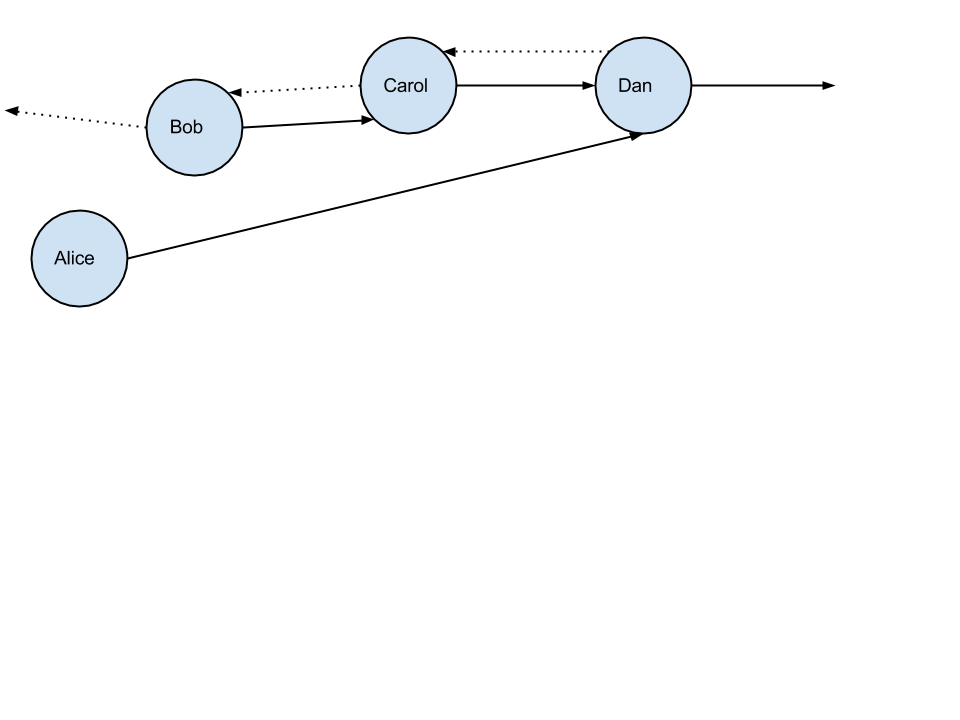
\includegraphics[width=\linewidth]{abcd1}
    \caption{Alice has incorrectly determined that Carol is her appropriate successor.  When Alice stabilizes, Carol will let her know about Bob.}
    \label{abcd1}
\end{figure}


\begin{figure}
    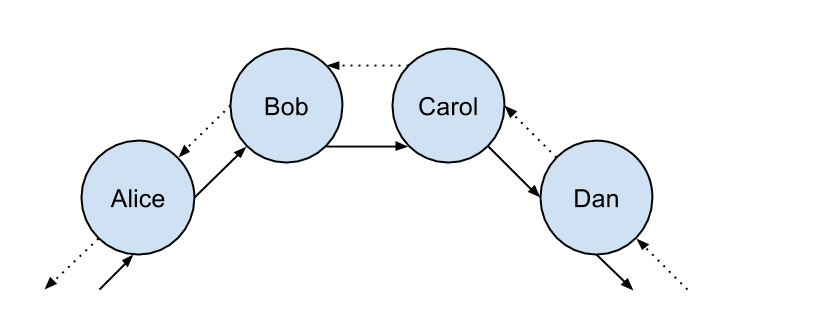
\includegraphics[width=\linewidth]{abcd2}
    \caption{After completing stabilize, Alice makes Bob her successor and notifies him. Bob then made Alice as his predecessor.}
    \label{abcd2}
\end{figure}



\subsubsection{Responsibility}
One of the major design choices for Chord implementation is not figuring which node is responsible for a given key, but figuring out who decides which node is responsible for a given key.

In our implementation, a node $n$ is responsible for the keys ($predecessor(n)$, $n$].  In other words, when $n$ gets a message, it considers itself the intended destination for the message if the message's destination hash is between $predecessor(n)$ and $n$.  A node that does not have a predecessor assigns itself as its own predecessor and considers itself responsible for all messages it receives.  COUNTER WHY THIS IS A BAD IDEA.  THIS IS A VERY DEFINITE CRITICISM 

When a node $n$ changes his successor, $n$ asks if the successor is holding any data $n$ should be responsible for.  The successor looks at all the data $n$ is better suited to hold onto, packages it up, and sends it along to $n$.  The successor does not have to delete this data. If fact, keeping this data as a backup is beneficial to the network as a whole, as $n$ could decide to leave the network at any poitn. 

\subsubsection{handling churn and politely quitting}
Due to the potentially volatile nature of a peer-to-peer network, Chord has to be able to handle (or at the very least, tolerate) an arbitrary amount of churn.  We already detailed how Chord gradually guides nodes into their correct locations after they join the network.  The same is true for when a node leaves the network; the stabilize procedure will guide nodes to their correct successors and predecessors.  However, we can exert more control over how to handle nodes leaving the network

A node can leave the ring in one of two ways.  A node can either suddenly drop out of existence, or a node can tell the network he is about to leave, letting his successor and predecessor immediately perform the needed changes.

When a node politely quits, he informs both his successor and predecessor and gives them all the information they need to correct \emph{their} predecessor and successor, respectively\footnote{This is not an easy to read explanation}. He also sends all of the data he is responsible for to his successor, who would become responsible for that data when that node left.  This allows for the network to adjust to the change with a minimum of fuss.

\subsubsection{the general idea of backup}
Unfortunately, it is impossible that every time a node leave the network it will do so politely.  If a node suddenly quits, the data it had stored goes with it. To prevent data from becoming irretrievable, a node can periodically send backups to its successor.  So as not to overwhelm the ring with a cascade of backups of backups, the node only passes along what it considers itself responsible for, which changes as nodes enter and leave the network.  If the backup leaves, he send his stuff to his successor, since the backup's successor would be the one responsible for the info now. 

\subsubsection{behavoir when a loses his predecessor or successor}


\section{MapReduce}
\subsubsection{History}

At its core, MapReduce \cite{mapreduce} is a system for division of labor.  One very popular implementation of MapReduce is  Apache's Hadoop. \cite{hadoop}.

\subsubsection{Example}

A task gets sent to a master node, who then divides that task among slave nodes, which may further divide the task.  This task has two distinct parts: Map and Reduce.  Map performs some operation on a set of data and then reduces a result for each map operation.  This intermediate data is then reduced by other slave nodes then returned to the user. 

The classic example given for MapReduce is counting the word in a collection of documents.  The master node splits up the documents into multiple chunks and sends them off to workers  \footnote{Workers can further split up the chunks among other workers.}.  Each worker then goes thru each chunk and creates a small word frequency list.  These lists are then used by other workers, who combine them into larger and larger lists, until the master node is left with a word frequency list of all the words in the documents. 



\subsubsection{Map Reduce advantages and disadvantages}
this is a good survey \cite{mrsurvey}.

\section{CHRONUS}


\subsection{Implementation}
Paragraph here about the bidding nature of the amazon market.
age of the inherent ring structure.





\subsubsection{Code Details}
We implemented the Chord based on the psuedocode  in the Stoica's paper \cite{Chord}, using Python instead of C++.  We also sent messages instead of performing remote procedure calls.


\subsubsection{Chunking}
We implemented two ways of storing a file.  The first is to store the whole file the node corresponding the hash of the file.  The second approach, presented  by Dabek ETAL \cite{CFS}, is to break the files into chunks.  Each chunk gets its own hash value and gets stored in the corresponding location.  To find these disparate  chunks, nodes retreive a \emph{key block}, which is stored at the location corresponding to the hash of the whole file.  This key block, when retrieved, tells the node the has value corresponding to the rest of the chunks.

The chunking allows for numerous advantages.  Each piece of the overall file would (ideally) be stored in a different node, each with a different backup.  This would prevent any single node from becoming overwhelmed from fulfilling multiple requests for a large file.  It would also prevent retrieval from being bottlenecked by a node with a relatively low bandwidth. Finally, When Chord uses some sort of caching scheme like that described in CFS \cite{CFS}, caching chunks as opposed to the entire file resulted in about 1000 times less storage overhead \footnote{this is duplicated text from another section on cfs}.  The results are likely similar with autonomous replication processes like IRM \cite{IRM}.

Chunking also opens up the options for implementing additional redundancy such as erasure codes\cite{rizzo1997effective}. With erasure codes, redundant chunks are created but any combination of a particular number of chunks is sufficient to recreate the file.  The additional redundency comes at the cost of using up more storage space and  the additional time needed to encode and decode the chunks.



\subsection{Distributed MapReduce}

\subsubsection{Operation}
In our implementation of a distributed map reduce, each node takes on responsibilities of both a worker and master, much in the same way that a node in a p2p file-sharing service will act as both a client and a server.  To start a job, the user contacts a node a specified hash address. The node he contacts to be the stager may be his own computer, and this is preferable when the job involves dividing up a large pile of data. 

The job of this stager is to take the work and divide it into \emph{data atoms}, which are the smallest individual units that work can be done on.  This might a line of text in a document, the result of a summation for a particular intermediate value, or a subset of items to be sorted.  The specifics of how to divide the work are defined by the user in a \emph{stage} function.  These \emph{data atoms} are then given a random hash and sent to that hash address, guaranteeing an even distribution of the data atoms throughout the network.  The \emph{data atoms} also contain the map function and reduce function, as defined by the user.

Nodes which receive data atoms apply the map function to the data to create intermediate data atoms, which are sent to other BLANK.  DESCRIBE HOW TWO INTERMEDIATE ATOMS GET TO THE SAME PLACE.  Nodes that receive at least two intermediate values merge them into one data atom using the reduce function.   The atoms are continually merged until only one remains at the hash address of the stager. 

Once the reductions are finished, the user gets his results from the node at the stager's address.

Once the stager has sent all the data atoms, his job is done.  The stager does not need to collect the results work, since the work is sent to the stager's hash address, rather than the stager itself.  Thus, the stager could quit the network after staging, and both the user and the network would be unaffected by the change.



\subsubsection{What happens if the stager goes down while staging} 

\subsubsection{Recap the issues  of normal MapReduce  and why ours is bettter} 
We present our implementation of MapReduce not as a direct competitor to MapReduce, but as proof of a more versatile system able to support many complex operations.

The big advantage of our system is the ease of development.  

The developer does not need to worry about distributing work evenly, nor does he have to worry about any node in the network going down.  The underlying Chord ring handles that automatically.  If a node joins the ring as the MapReduce process is running, that node can be assigned work automatically.  The stager does not need to keep track of the status of the network.  In a node goes down while performing an operation, his sucessor takes over for him.

All a developer needs to do to write three functions: the staging function, map, and reduce.  These define how to split up the work into managable portions,  the  work to be performed on each portion to get some results, and how to combine these results into a single result. 

In the next section, we show two of the implenations we ran on our ring of nodes.

\subsection{Example implementations of mapreduce}

\subsubsection{Calculating Pi}

\subsubsection{Word Count}

\subsection{In which we address possible criticism}




\subsubsection{If we hash a filename to get the identifier, then you can't have two same file names.}
\subsubsection{Determining when you're done is expensive}
As a whole yes, but merging two sorted lists is $O(n)$ time. 


\subsubsection{Disjoint rings}
We can assign every node a \emph{ring id}.  When a node creates a ring, he randomly chooses a number for the ring id.  Nodes joining that ring use that ring's id.  If a node finds another node on differing ring, he compares the their ring id's and leaves if  

\subsubsection{The security we didn't do}
We can have multiple non interacting secure file systems.


\section{Experiments}
A set of experiments were run on large groups of Amazon EC2 Micro Instances\cite{amazon-micro}.

We ran word count on James Joyce's \emph{Ulysses} \cite{joyce1924ulysses}.


 
\section{Results}

\section{Conclusion}
Our stuff \cite{code} is awesome.

\bibliographystyle{plain}
\bibliography{CHRONUS}
\end{document}
